% FIGURE LIST

%%%%%%% MAIN FIGURES %%%%%%%
% DESIGN

\newcommand{\FigDesign}{
  \begin{figure}[H]
    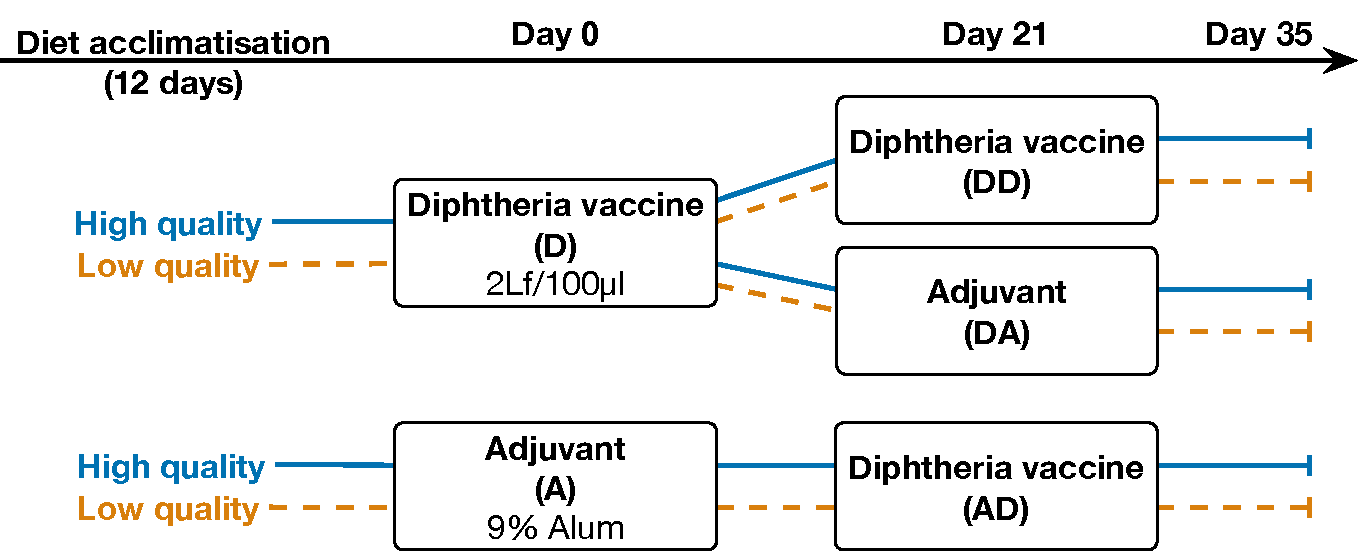
\includegraphics[width=1\textwidth, keepaspectratio=true]{./Figures/Apodemus-vacc-figures/StudyDesign_paper.pdf}
    \caption{\textbf{Allocation of diet and vaccines.} Wood mice from a laboratory colony, and from the wild were provided enriched (TransBreed) or standard (lab: normal chow; wild: no supplementation) diets. After at least 12 days, mice were allocated at random to immunisation with a 2Lf/100µl Diphtheria Toxoid + 9\% alum vaccine (D) or with adjuvant alone (A). Twenty-one days after their first immunisation, mice that had been immunised with D were then given a second shot of the vaccine (DD) or adjuvant alone (DA), while mice that had received an initial adjuvant vaccine (A) were all given D for their second shot (AD).}
    \label{fig:design}
  \end{figure}
}

% ELISA

\newcommand{\FigIgG}{
  \begin{figure}[hp]

    
\includegraphics[width=\textwidth, keepaspectratio=true]{./Figures/plots/IgG1.pdf}

    \caption{\textbf{Vaccine-induced DTV-specific IgG1.} \textbf{A}, diphtheria toxoid vaccine (DTV)-specific IgG1 optical density in mice from laboratory- and wild-habitats provided high and low quality dietary supplements. Mice were immunised either once, with adjuvant as control (A) or DTV (D), or twice, using adjuvant alone followed by DTV (AD), DTV and subsequently adjuvant alone (DA), or two separate doses of DTV (DD). Only mice immunised at least 7 days prior to serum ELISA sampling are shown. \textbf{B}, posterior conditional distributions of the coefficients for diet, habitat, and vaccine formulation (A, D, AD, DA, DD), and effect of the same vaccines. Each density curve represents the distribution of 3,000 samples from one of four MCMC chains; dotted line represents the the value for which the reference (global intercept for Diet and Habitat; Adjuvant alone for the vaccines) is null (see parameter estimates in Table~\ref{tbl:precis}).}

    \label{fig:igg1}

  \end{figure}
}

% DAG

\newcommand{\FigDAGtikz}{
  \begin{figure}
    \centering
    % This code uses the tikz package
    % \documentclass{standalone}
% \usepackage[dvipsnames]{xcolor}
% \usepackage{tikz}
% \usetikzlibrary{arrows.meta}

% \begin{document}

\tikzstyle{mybox} = [inner sep=1pt]

% Top row: A and B
\begin{subfigure}[t]{0.47\textwidth}
    % Panel A
    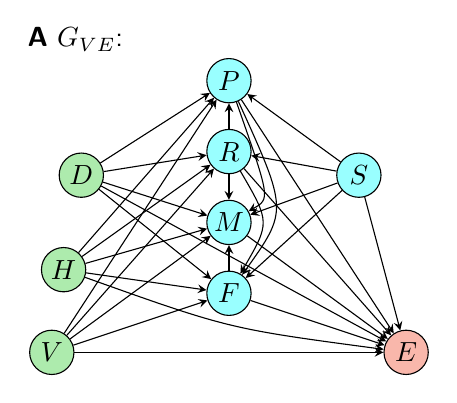
\begin{tikzpicture}[scale=0.75, inner sep=0pt]
      \node[inner sep = 0, font=\sffamily] (panel A) at (-2.6,5.3) {\textbf{A} $\mathbb{G}_{VE}$:};
      \node[circle, draw, fill=LimeGreen, text opacity=1, fill opacity=0.4, minimum width=16pt] (V) at (-3,0) {\(V\)};
      \node[circle, draw, fill=RedOrange, text opacity=1, fill opacity=0.4, minimum width=16pt] (E) at (3,0) {\(E\)};
      \node[circle, draw, fill=LimeGreen, text opacity=1, fill opacity=0.4, minimum width=16pt] (H) at (-2.8,1.4) {\(H\)};
      \node[circle, draw, fill=LimeGreen, text opacity=1, fill opacity=0.4, minimum width=16pt] (D) at (-2.5,3) {\(D\)};
      \node[circle, draw, fill=Cyan, text opacity=1, fill opacity=0.4, minimum width=16pt] (F) at (0,1) {\(F\)};
      \node[circle, draw, fill=Cyan, text opacity=1, fill opacity=0.4, minimum width=16pt] (M) at (0,2.2) {\(M\)};
      \node[circle, draw, fill=Cyan, text opacity=1, fill opacity=0.4, minimum width=16pt] (R) at (0,3.4) {\(R\)};
      \node[circle, draw, fill=Cyan, text opacity=1, fill opacity=0.4, minimum width=16pt] (P) at (0,4.6) {\(P\)};
      \node[circle, draw, fill=Cyan, text opacity=1, fill opacity=0.4, minimum width=16pt] (S) at (2.2,3) {\(S\)};

      % Edges from D
      \draw [-stealth] (D) edge (E);
      \draw [-stealth] (D) edge (F);
      \draw [-stealth] (D) edge (M);
      \draw [-stealth] (D) edge (P);
      \draw [-stealth] (D) edge (R);

      % Edges from F
      \draw [-stealth] (F) edge (E);
      \draw [-stealth] (F) edge (M);

      % Edges from M
      \draw [-stealth] (M) edge (E);

      % Edges from P
      \draw [-stealth] (P) edge (E);
      \draw [-stealth] (P) .. controls (1, 2.4) .. (F);
      \draw [-stealth] (P) .. controls (0.7, 2.6) .. (M);

      % Edges from R
      \draw [-stealth] (R) edge (E);
      \draw [-stealth] (R) .. controls (0.7, 2.2) .. (F);
      \draw [-stealth] (R) edge (M);
      \draw [-stealth] (R) edge (P);

      % Edges from S
      \draw [-stealth] (S) edge (E);
      \draw [-stealth] (S) edge (F);
      \draw [-stealth] (S) edge (M);
      \draw [-stealth] (S) edge (P);
      \draw [-stealth] (S) edge (R);

      % Edges from V
      \draw [-stealth] (V) edge (E);
      \draw [-stealth] (V) edge (F);
      \draw [-stealth] (V) edge (M);
      \draw [-stealth] (V) edge (R);
      \draw [-stealth] (V) edge (P);

      % Edges from H
      \draw [-stealth] (H) .. controls (0, 0.4) .. (E);
      \draw [-stealth] (H) edge (F);
      \draw [-stealth] (H) edge (M);
      \draw [-stealth] (H) edge (P);
      \draw [-stealth] (H) edge (R);
    \end{tikzpicture}
\end{subfigure}
\hspace{-5em}
\begin{subfigure}[t]{0.47\textwidth}
    % Panel B
    \begin{tikzpicture}
      \node[inner sep = 0, font=\sffamily] (panel B) at (4.3,2.2) {\textbf{B} $\mathbb{C}_{VE}$:};
      \node [mybox, right =of E] (box){%
        \begin{minipage}[!t]{\textwidth}
          \footnotesize
          \openup -0.5ex
          \begin{equation} \label{eq:SCM_fig}
            \begin{aligned}
          V &\coloneq \mathcal{U}_V \\
          H &\coloneq \mathcal{U}_H \\
          D &\coloneq \mathcal{U}_D \\
          S &\coloneq \mathcal{U}_S \\
          R &\coloneq f_R(V, H, D, S, \mathcal{U}_R) \\
          P &\coloneq f_P(V, H, D, S, R, \mathcal{U}_P) \\
          F &\coloneq f_F(V, H, D, S, P, R, \mathcal{U}_F) \\
          M &\coloneq f_M(V, H, D, S, P, R, F, \mathcal{U}_M) \\
          E &\coloneq f_E(V, H, D, S, P, R, M, F, \mathcal{U}_E) \\
          \end{aligned}
          \end{equation}
        \end{minipage}
      };
    \end{tikzpicture}
\end{subfigure}

% Add vertical space between rows
\vspace{1em}

% Bottom row: C and D
\begin{subfigure}[t]{0.47\textwidth}
    % Panel C
    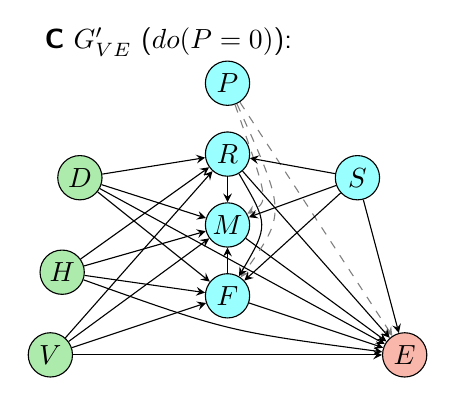
\begin{tikzpicture}[scale=0.75, inner sep=0pt, xshift=-1cm]
      \node[inner sep = 0, font=\sffamily] (panel C) at (-1,5.3) {\textbf{C} $\mathbb{G}'_{VE}$ ($do(P=0)$):};
      \node[circle, draw, fill=LimeGreen, text opacity=1, fill opacity=0.4, minimum width=16pt] (V) at (-3,0) {\(V\)};
      \node[circle, draw, fill=RedOrange, text opacity=1, fill opacity=0.4, minimum width=16pt] (E) at (3,0) {\(E\)};
      \node[circle, draw, fill=LimeGreen, text opacity=1, fill opacity=0.4, minimum width=16pt] (H) at (-2.8,1.4) {\(H\)};
      \node[circle, draw, fill=LimeGreen, text opacity=1, fill opacity=0.4, minimum width=16pt] (D) at (-2.5,3) {\(D\)};
      \node[circle, draw, fill=Cyan, text opacity=1, fill opacity=0.4, minimum width=16pt] (F) at (0,1) {\(F\)};
      \node[circle, draw, fill=Cyan, text opacity=1, fill opacity=0.4, minimum width=16pt] (M) at (0,2.2) {\(M\)};
      \node[circle, draw, fill=Cyan, text opacity=1, fill opacity=0.4, minimum width=16pt] (R) at (0,3.4) {\(R\)};
      \node[circle, draw, fill=Cyan, text opacity=1, fill opacity=0.4, minimum width=16pt] (P) at (0,4.6) {\(P\)};
      \node[circle, draw, fill=Cyan, text opacity=1, fill opacity=0.4, minimum width=16pt] (S) at (2.2,3) {\(S\)};

      % Edges from D
      \draw [-stealth] (D) edge (E);
      \draw [-stealth] (D) edge (F);
      \draw [-stealth] (D) edge (M);
      % \draw [-stealth, dashed, gray] (D) edge (P);
      \draw [-stealth] (D) edge (R);

      % Edges from F
      \draw [-stealth] (F) edge (E);
      \draw [-stealth] (F) edge (M);

      % Edges from M
      \draw [-stealth] (M) edge (E);

      % Edges from P
      \draw [-stealth, dashed, gray] (P) edge (E);
      \draw [-stealth, dashed, gray] (P) .. controls (1, 2.4) .. (F);
      \draw [-stealth, dashed, gray] (P) .. controls (0.7, 2.6) .. (M);

      % Edges from R
      \draw [-stealth] (R) edge (E);
      \draw [-stealth] (R) .. controls (0.7, 2.2) .. (F);
      \draw [-stealth] (R) edge (M);
      % \draw [-stealth, dashed, gray] (R) edge (P);

      % Edges from S
      \draw [-stealth] (S) edge (E);
      \draw [-stealth] (S) edge (F);
      \draw [-stealth] (S) edge (M);
      % \draw [-stealth, dashed, gray] (S) edge (P);
      \draw [-stealth] (S) edge (R);

      % Edges from V
      \draw [-stealth] (V) edge (E);
      \draw [-stealth] (V) edge (F);
      \draw [-stealth] (V) edge (M);
      \draw [-stealth] (V) edge (R);
      % \draw [-stealth, dashed, gray] (V) edge (P);

      % Edges from H
      \draw [-stealth] (H) .. controls (0, 0.4) .. (E);
      \draw [-stealth] (H) edge (F);
      \draw [-stealth] (H) edge (M);
      % \draw [-stealth, dashed, gray] (H) edge (P);
      \draw [-stealth] (H) edge (R);
    \end{tikzpicture}
\end{subfigure}%
\hspace{-5em}
\begin{subfigure}[t]{0.49\textwidth}
    % Panel D
    \begin{tikzpicture}
      \node[inner sep = 5, font=\sffamily] (panel D) at (4.3,2.3) {\textbf{D} $\mathbb{C}'_{VE}$ ($do(P=0)$):};
      \node [mybox, right =of E] (box){%
        \begin{minipage}[!t]{\textwidth}
          \footnotesize
          \openup -0.5ex
          \begin{equation} \label{eq:SCMcounterfactual_fig}
            \begin{aligned}
          P & = 0 \\
          V & \coloneq \mathcal{U}_V \\
          H & \coloneq \mathcal{U}_H \\
          D & \coloneq \mathcal{U}_D \\
          S & \coloneq \mathcal{U}_S \\
          R & \coloneq f_R(V, H, D, S, \mathcal{U}_R) \\
          F & \coloneq f_F^{P=0}(V, H, D, S, R, \mathcal{U}_F) \\
          M & \coloneq f_M^{P=0}(V, H, D, S, R, F, \mathcal{U}_M) \\
          E & \coloneq f_E^{P=0}(V, H, D, S, R, M, F, \mathcal{U}_E) \\
          \end{aligned}
          \end{equation}
        \end{minipage}
      };
    \end{tikzpicture}
\end{subfigure}

% \end{document}

    \caption{\textbf{Causal Model of vaccine responsiveness.} \textbf{A}, Directed acyclic graph $\mathbb{G}_{VE}$ representing hypothesised causal effects driving variation in efficacy \(E\) of vaccine \(V\) in laboratory or wild mice \(H\), under supplemented or control diet \(D\) (green nodes depict experimental treatments). Covariates, mediators, and potential confounders (blue nodes) were time since vaccination \(T\), parasite infection (presence or burden) \(P\), reproductive status \(R\), body mass \(M\), fat scores \(F\), and sex \(S\). Directed edges depict causal effects hypothesised to operate between nodes. \textbf{B}, Structural causal model \(\mathbb{C}_{VE}\) derived from $\mathbb{G}_{VE}$ with coefficients $\beta_{ij}$ representing the effect of cause $i$ on effect $j$. $\mathcal{U}_j$ represents the unmeasured variation of the response variable, not represented in $\mathbb{G}_{VE}$ (panel A) for clarity.}

    \label{fig:DAGtikz}
  \end{figure}
}

\newcommand{\FigDAGtikzParam}{
  \begin{figure}
    \centering
    % This code uses the tikz package
    % \documentclass{standalone}
% \usepackage[dvipsnames]{xcolor}
% \usepackage{tikz}
\usetikzlibrary{arrows.meta}

% \begin{document}
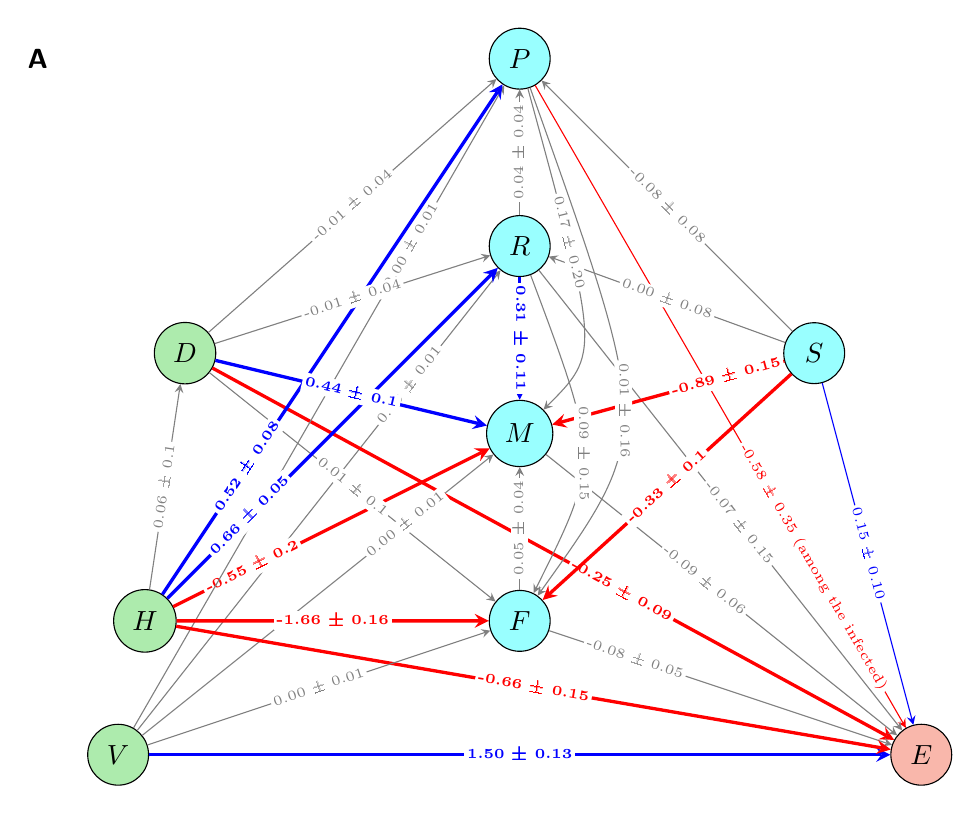
\begin{tikzpicture}[scale=1.7]
	\node[inner sep = 0, font=\sffamily] (panel A) at (-3.6,5.2) {\textbf{A}};
	\node[circle, draw, inner sep=4pt, fill=LimeGreen, font=\bfseries, text opacity=1, fill opacity=0.4, minimum width=22pt] (V) at (-3,0) {\(V\)};
	\node[circle, draw, inner sep=4pt, fill=RedOrange, font=\bfseries, text opacity=1, fill opacity=0.4, minimum width=22pt] (E) at (3,0) {\(E\)};
	\node[circle, draw, inner sep=4pt, fill=LimeGreen, font=\bfseries, text opacity=1, fill opacity=0.4, minimum width=22pt] (H) at (-2.8,1) {\(H\)};
	\node[circle, draw, inner sep=4pt, fill=LimeGreen, font=\bfseries, text opacity=1, fill opacity=0.4, minimum width=22pt] (D) at (-2.5,3) {\(D\)};
	\node[circle, draw, inner sep=4pt, fill=Cyan, font=\bfseries, text opacity=1, fill opacity=0.4, minimum width=22pt] (F) at (0,1) {\(F\)};
	\node[circle, draw, inner sep=4pt, fill=Cyan, font=\bfseries, text opacity=1, fill opacity=0.4, minimum width=22pt] (M) at (0,2.4) {\(M\)};
	\node[circle, draw, inner sep=4pt, fill=Cyan, font=\bfseries, text opacity=1, fill opacity=0.4, minimum width=22pt] (R) at (0,3.8) {\(R\)};
	\node[circle, draw, inner sep=4pt, fill=Cyan, font=\bfseries, text opacity=1, fill opacity=0.4, minimum width=22pt] (P) at (0,5.2) {\(P\)};
	\node[circle, draw, inner sep=4pt, fill=Cyan, font=\bfseries, text opacity=1, fill opacity=0.4, minimum width=22pt] (S) at (2.2,3) {\(S\)};

	\draw [-stealth, gray] (V) -- (R) node[near end, font=\tiny,
		fill=white, sloped, inner sep=1] {0.00 ± 0.01};
	\draw [-stealth, red, very thick] (H) -- (M) node[near start, font=\tiny\bfseries, text=red,
		fill=white, sloped, inner sep=1] {-0.55 ± 0.2};
	\draw [-stealth, red, very thick] (D) -- (E) node[pos=0.6, font=\tiny\bfseries, text=red,
		fill=white, sloped, inner sep=1] {-0.25 ± 0.09};
	\draw [-stealth, gray] (D) -- (F) node[midway, font=\tiny,
		fill=white, sloped, inner sep=1] {0.01 ± 0.1};
	\draw [-stealth, gray] (D) -- (P) node[midway, font=\tiny,
		fill=white, sloped, inner sep=1] {-0.01 ± 0.04};
	\draw [-stealth, gray] (F) -- (E) node[near start, font=\tiny,
		fill=white, sloped, inner sep=1] {-0.08 ± 0.05};
	\draw [-stealth, gray] (F) -- (M) node[midway, font=\tiny,
		fill=white, sloped, inner sep=1] {0.05 ± 0.04};
	\draw [-stealth, gray] (M) -- (E) node[pos=0.45, font=\tiny,
		fill=white, sloped, inner sep=1] {-0.09 ± 0.06};
	\draw [-stealth, red] (P) -- (E) node[near end, font=\tiny,
		fill=white, sloped, inner sep=1] {-0.58 ± 0.35 (among the infected)};
	\draw [-stealth, gray] (R) -- (E) node[pos=0.55, font=\tiny,
		fill=white, sloped, inner sep=1] {-0.07 ± 0.15};
	\draw [-stealth, blue, very thick] (R) -- (M) node[midway, font=\tiny\bfseries, text=blue,
		fill=white, sloped, inner sep=1] {0.31 ± 0.11};
	\draw [-stealth, gray] (R) -- (P) node[midway, font=\tiny,
		fill=white, sloped, inner sep=1] {0.04 ± 0.04};
	\draw [-stealth, blue] (S) -- (E) node[midway, font=\tiny,
		fill=white, sloped, inner sep=1] {0.15 ± 0.10};
	\draw [-stealth, red, very thick] (S) -- (F) node[midway, font=\tiny\bfseries, text=red,
		fill=white, sloped, inner sep=1] {-0.33 ± 0.1};
	\draw [-stealth, red, very thick] (S) -- (M) node[near start, font=\tiny\bfseries, text=red,
		fill=white, sloped, inner sep=1] {-0.89 ± 0.15};
	\draw [-stealth, gray] (S) -- (P) node[midway, font=\tiny,
		fill=white, sloped, inner sep=1] {-0.08 ± 0.08};
	\draw [-stealth, gray] (S) -- (R) node[midway, font=\tiny,
		fill=white, sloped, inner sep=1] {0.00 ± 0.08};
	\draw [-stealth, gray] (V) -- (M) node[near end, font=\tiny,
		fill=white, sloped, inner sep=1] {0.00 ± 0.01};
	\draw [-stealth, gray] (V) -- (P) node[near end, font=\tiny,
		fill=white, sloped, inner sep=1] {0.00 ± 0.01};
	\draw [-stealth, blue, very thick] (V) -- (E) node[midway, font=\tiny\bfseries, text=blue,
		fill=white, sloped, inner sep=1] {1.50 ± 0.13};
	\draw [-stealth, gray] (H) -- (D) node[midway, font=\tiny,
		fill=white, sloped, inner sep=1] {0.06 ± 0.1};
	\draw [-stealth, red, very thick] (H) -- (E) node[midway, font=\tiny\bfseries, text=red,
		fill=white, sloped, inner sep=1] {-0.66 ± 0.15};
	\draw [-stealth, red, very thick] (H) -- (F) node[midway, font=\tiny\bfseries, text=red,
		fill=white, sloped, inner sep=1] {-1.66 ± 0.16};
	\draw [-stealth, blue, very thick] (H) -- (P) node[near start, font=\tiny\bfseries, text=blue,
		fill=white, sloped, inner sep=1] {0.52 ± 0.08};
	\draw [-stealth, blue, very thick] (H) -- (R) node[near start, font=\tiny\bfseries, text=blue,
		fill=white, sloped, inner sep=1] {0.66 ± 0.05};
	\draw [-stealth, blue, very thick] (D) -- (M) node[midway, font=\tiny\bfseries, text=blue,
		fill=white, sloped, inner sep=1] {0.44 ± 0.1};
	\draw [-stealth, gray] (R) .. controls (0.6, 2.2) .. (F) node[midway, font=\tiny,
			fill=white, sloped, inner sep=1] {0.09 ± 0.15};
	\draw [-stealth, gray] (P) .. controls (1, 2.4) .. (F) node[midway, font=\tiny,
			fill=white, sloped, inner sep=1] {0.01 ± 0.16};
	\draw [-stealth, gray] (P) .. controls (0.6, 3) .. (M) node[near start, font=\tiny,
			fill=white, sloped, inner sep=1] {0.17 ± 0.20};
	\draw [-stealth, gray] (V) -- (F) node[midway, font=\tiny,
		fill=white, sloped, inner sep=1] {0.00 ± 0.01};
	\draw [-stealth, gray] (D) -- (R) node[midway, font=\tiny,
		fill=white, sloped, inner sep=1] {-0.01 ± 0.04};
\end{tikzpicture}

% \vspace{0.1cm}

\begin{tikzpicture}
	\node[inner sep=0pt, left of = V, align=left] (probs)
	{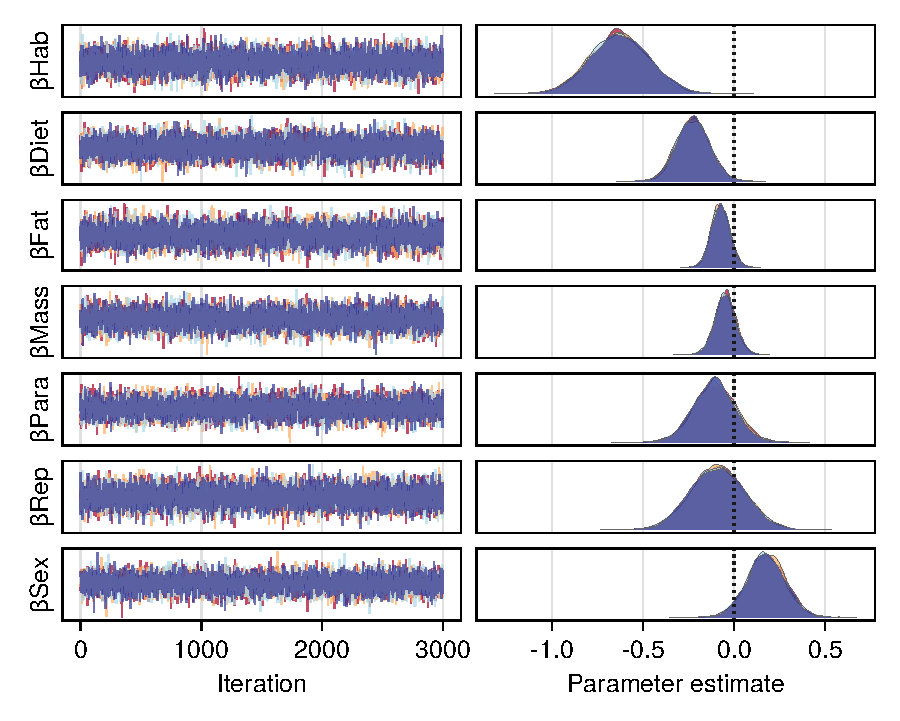
\includegraphics[width=0.8\textwidth]{./Figures/plots/MultiLevel_DE_H_E_chn_traces.pdf}};
	\node[inner sep = 0, font=\sffamily, align=left] (panel A) at (-12,4.5) {\textbf{B}};
\end{tikzpicture}
% \end{document}

    \caption{\textbf{Fully resolved Causal Model of vaccine efficacy.} \textbf{A}, Directed acyclic graph representing point estimates of positive (blue) and negative (red) direct causal effects ± std driving vaccine responsiveness \(E\). \textbf{B}, MCMC sampling of posterior distributions of the coefficients estimating the direct effect of the wild habitat $H$ on vaccine responsiveness $E$, with the adjustment set including, Diet $D$, Fat scores $F$, body mass $M$, parasite burden $P$, active reproductive status $R$, and female sex $S$; vaccine formulation $V$ and individual treated as random effects:
      $E \coloneq β_{Hab}H + β_{Diet}D + β_{Fat}F + β_{Mass}M + β_{Para}P + β_{Rep}R + β_{Sex}S + \mathcal{N}(0,Exp(\sigma_E))$
    (see \nameref{sec:parameterisation} methods). Note that each edge in panel A shows the direct causal effect of its parent node on its child node, which is conditional on the specific adjustment set for that model; thus, only the coefficient $β_{Diet}$ for the edge between $D$ and $E$ is a causal estimate in panel B, while the others are only associative.}
    \label{fig:DAGtikzParam}
  \end{figure}
}

\newcommand{\FigDAG}{
  \begin{figure}
    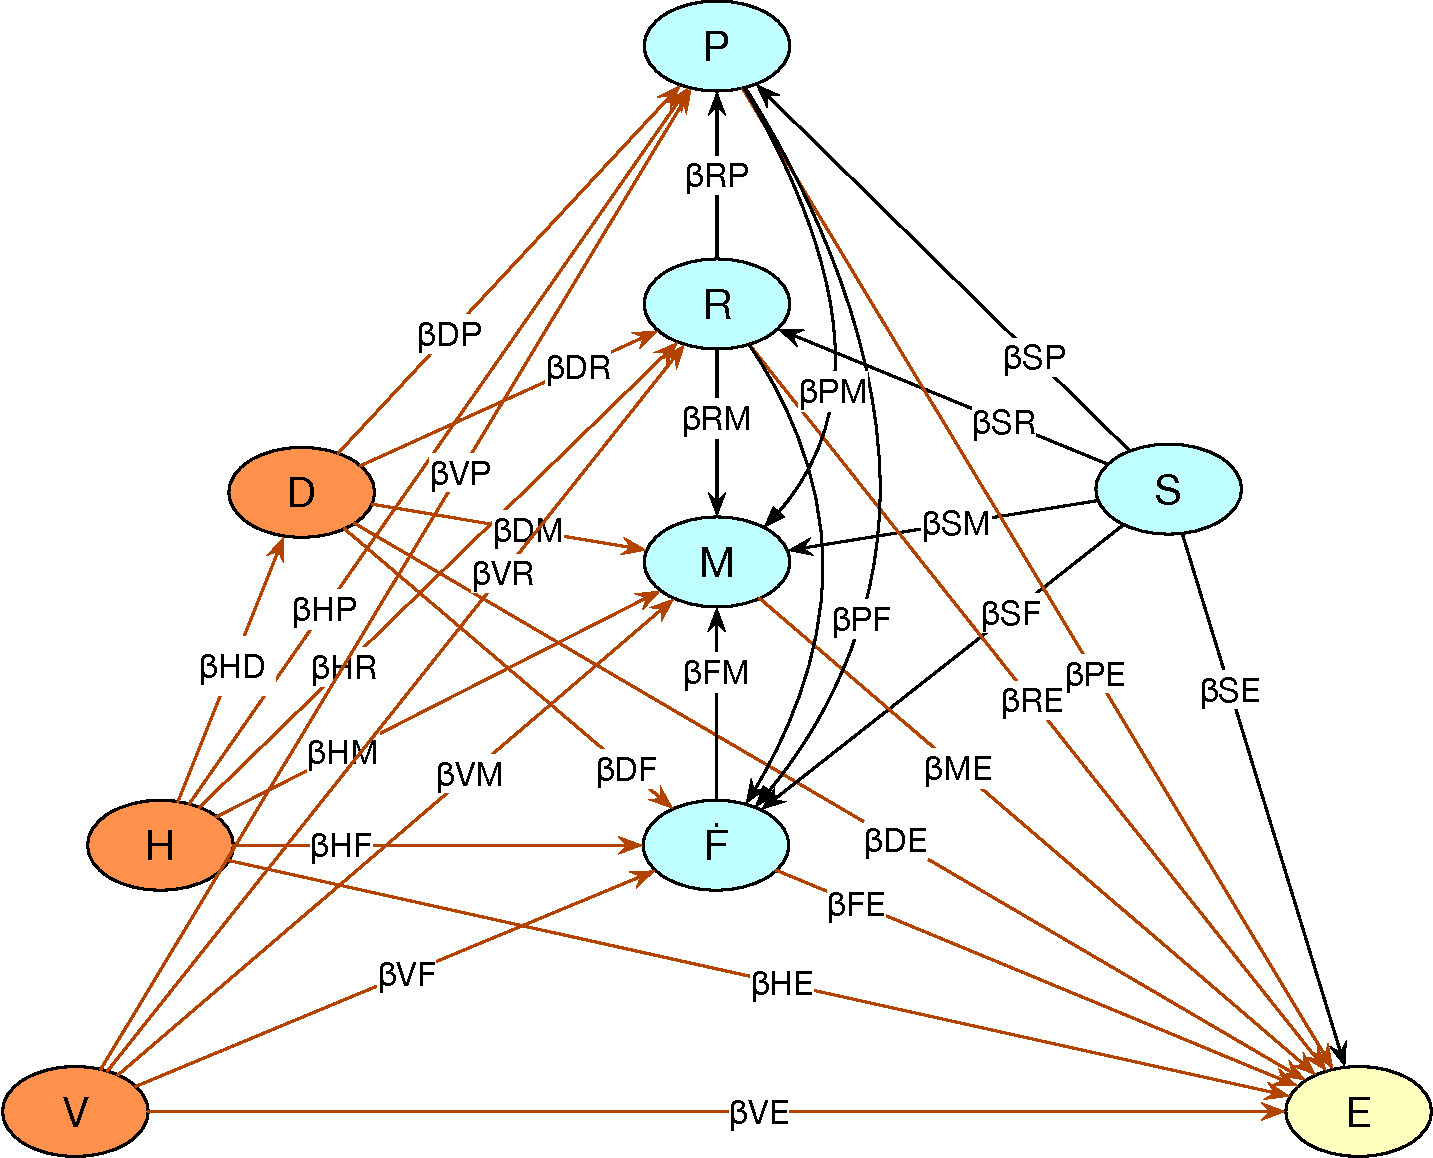
\includegraphics[width=\textwidth, keepaspectratio=true]{./Figures/Apodemus-vacc-figures/DAG.pdf}
    \caption{\textbf{Graphical Causal Model of vaccine efficacy.} Directed acyclic graph representing validated causal relationships expressed by the SCM \(\mathbb{C}_{VE}\) (Model~\ref{eq:SCM}). Covariates and potential confounders (blue nodes) were time since vaccination \(T\), parasite infection (presence or burden) \(P\), reproductive status \(R\), body mass \(M\), fat scores \(F\), and sex \(S\). }
    \label{fig:DAG}
  \end{figure}
}

\newcommand{\FigHabitat}{
  \begin{figure}[hp]
    \centering

    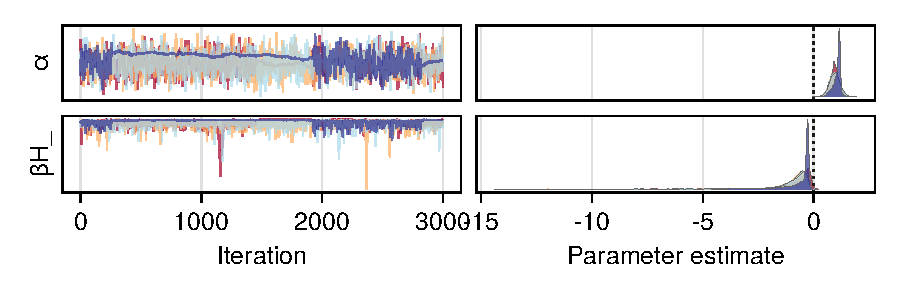
\includegraphics[width=0.7\textwidth, keepaspectratio=true]{./Figures/plots/H_E_chn.pdf}

    \caption{\textbf{Total causal effect of the wild habitat on vaccine responsiveness.}}

    \label{fig:habitat}

  \end{figure}
}

\newcommand{\FigDiet}{
  \begin{figure}[hp]
    \centering

    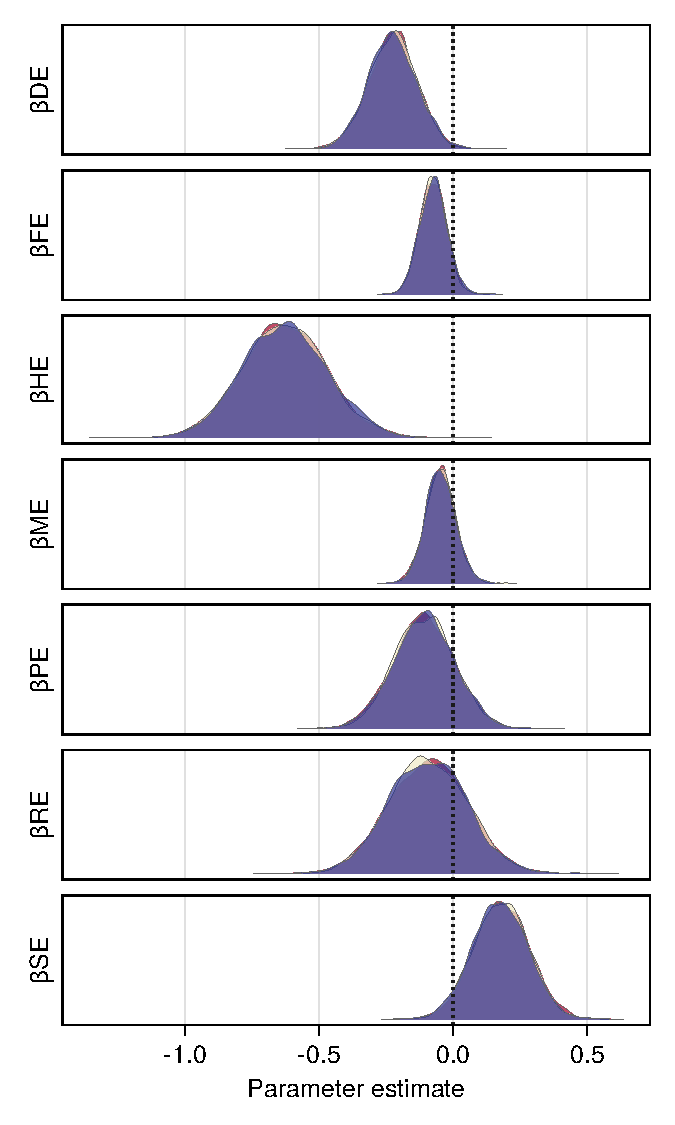
\includegraphics[width=0.5\textwidth, keepaspectratio=true]{./Figures/plots/MultiLevel_DE_D_E_chn.pdf}

    \caption{\textbf{Natural direct causal effect of diet etc. on vaccine responsiveness.}}

    %        \label{fig:diet}

  \end{figure}
}

\newcommand{\FigParasite}{
  \begin{figure}[hp]
    \centering

    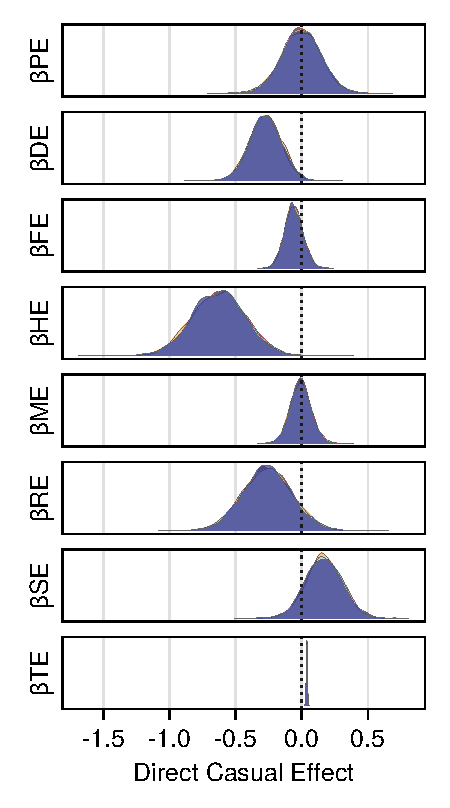
\includegraphics[width=0.5\textwidth, keepaspectratio=true]{./Figures/plots/MultiLevel_NDE_P_E_chn.pdf}

    \caption{\textbf{Natural direct causal effect of parasite burden, etc. on vaccine responsiveness.}}

    \label{fig:parasite}

  \end{figure}
}

\newcommand{\FigPostAnthelminthic}{
  \begin{figure}[H]
    \centering
    \begin{subfigure}[b]{0.5\textwidth}
      \centering
      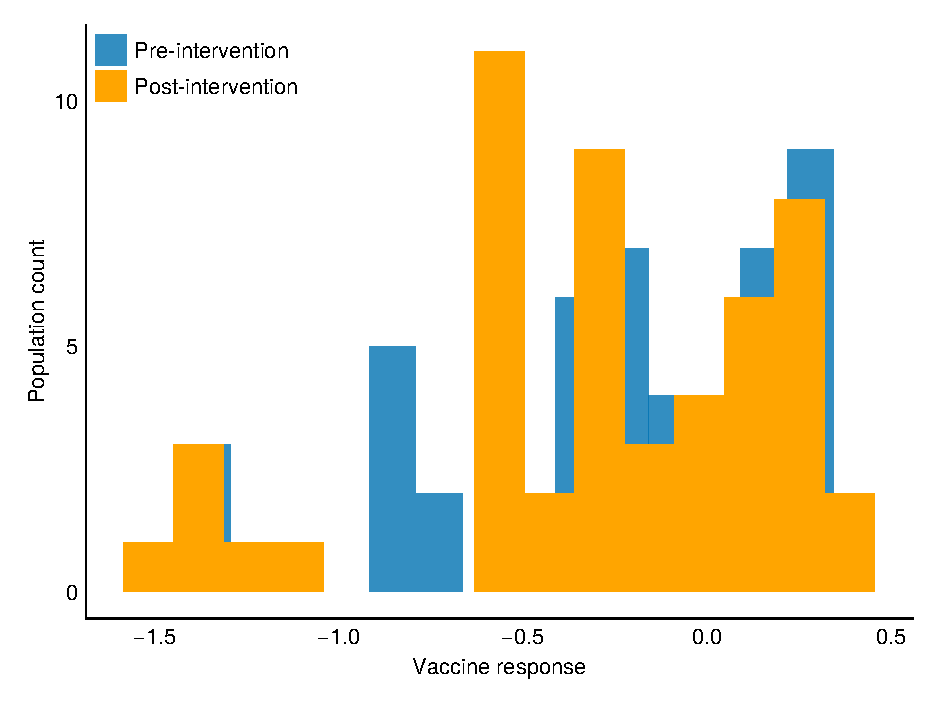
\includegraphics[width=\textwidth, keepaspectratio=true]{./Figures/plots/E_pre_post.pdf}
      \put(-200, 160){\sffamily \textbf{A}} % Adjust coordinates as needed
    \end{subfigure}%
    \begin{subfigure}[b]{0.5\textwidth}
      \centering
      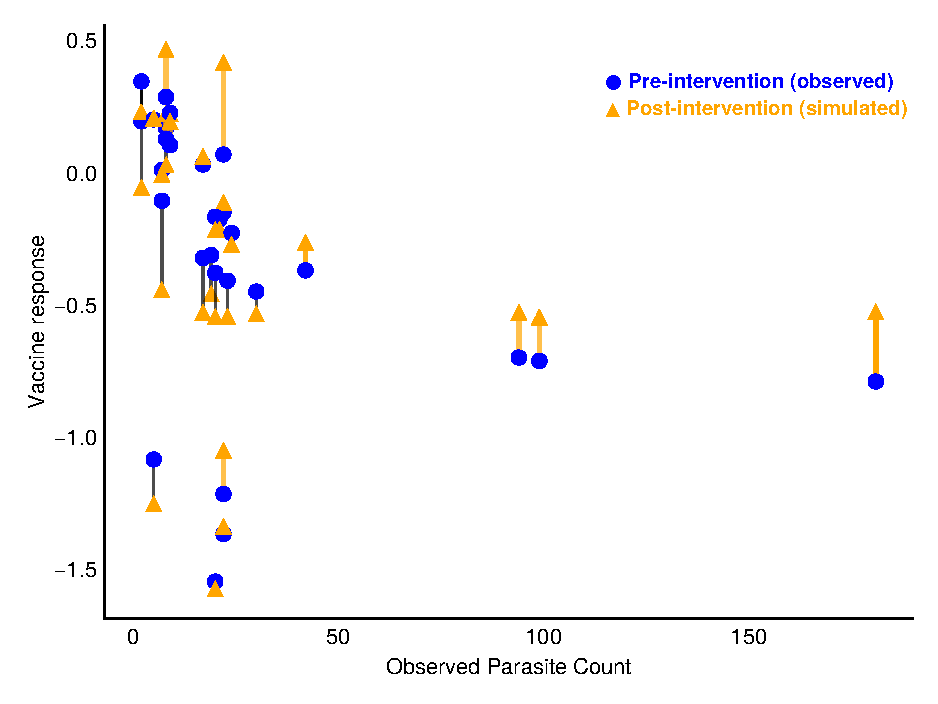
\includegraphics[width=\textwidth, keepaspectratio=true]{./Figures/plots/post_anthelminthic_effect_on_E.pdf}
      \put(-200, 160){\sffamily \textbf{B}} % Adjust coordinates as needed
    \end{subfigure}
    \caption{\textbf{Effect of simulated population-wide anthelmintic intervention on vaccine responsiveness.} \textbf{A}, Effect on population-wide vaccine responsiveness. \textbf{B}, Effect on individual vaccine responsiveness as a function of pre-intervention parasite burden.}
    \label{fig:post_anthelminthic}
  \end{figure}
}

%%%%%%% SUPPLEMENTARY FIGURES %%%%%%%

\newcommand{\SupFigSCMFlow}{
  \begin{figure}[hp]
    \centering
    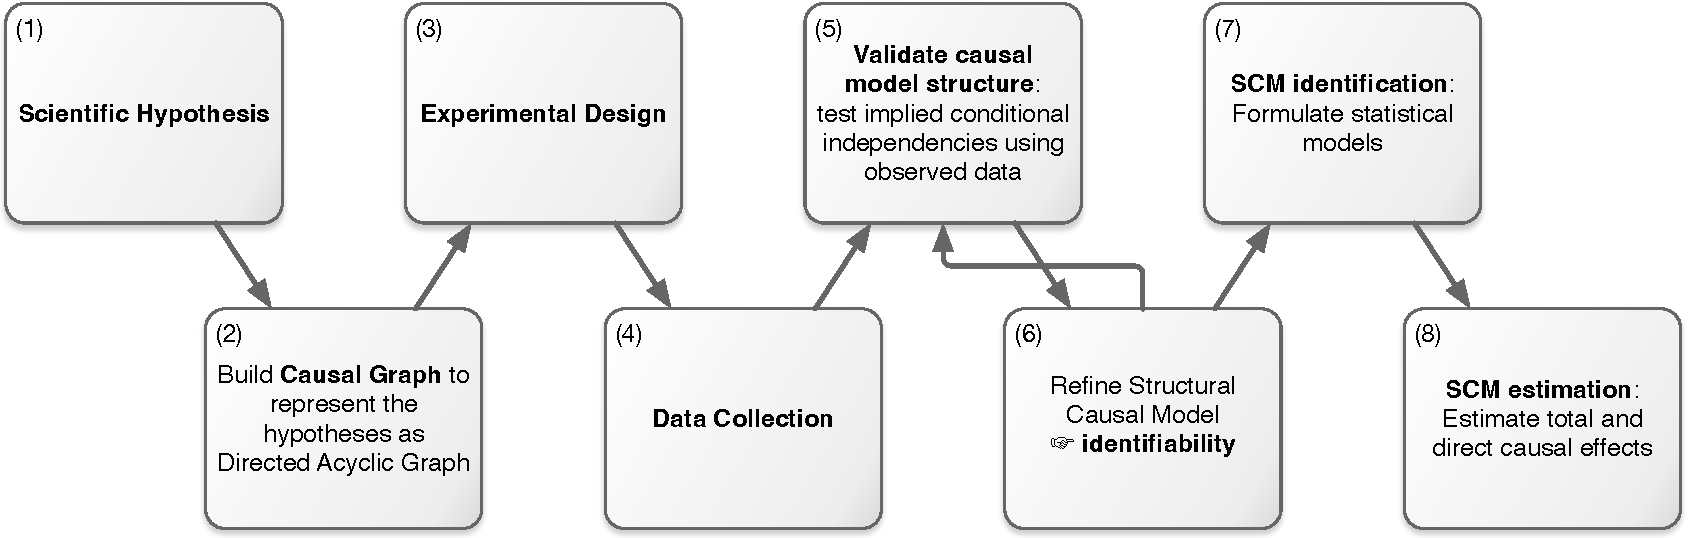
\includegraphics[width=1\textwidth, keepaspectratio=true]{./Figures/Apodemus-vacc-figures/SCM_flow.pdf}
    \caption{\textbf{Flow diagram of the SCM.} The Structural Causal Model (SCM) process explicitly represents scientific hypotheses (1) as a directed acyclic graph (DAG). This DAG is mathematically encoded as a set of nested equations that describe the flow of causation between variables, and helps inform lab and field experimental design (3) and data collection (4). After processing, the data are used to test the validity of the causal assumptions underlying the SCM, e.g. by testing the conditional independencies implied by the DAG (5). If the assumptions are not supported, refinements of the SCM (6) are necessary. When all conditions are met, the SCM is identifiable and statistical models can be formulated to adjust for confounding (7). Parameters from these models can then be used as estimates of direct and indirect causal effects (8).
    }
    \label{supfig:SCM_flow}
  \end{figure}
}

\newcommand{\SupFigMCMCChainIgG}{
  \begin{figure}[hp]

    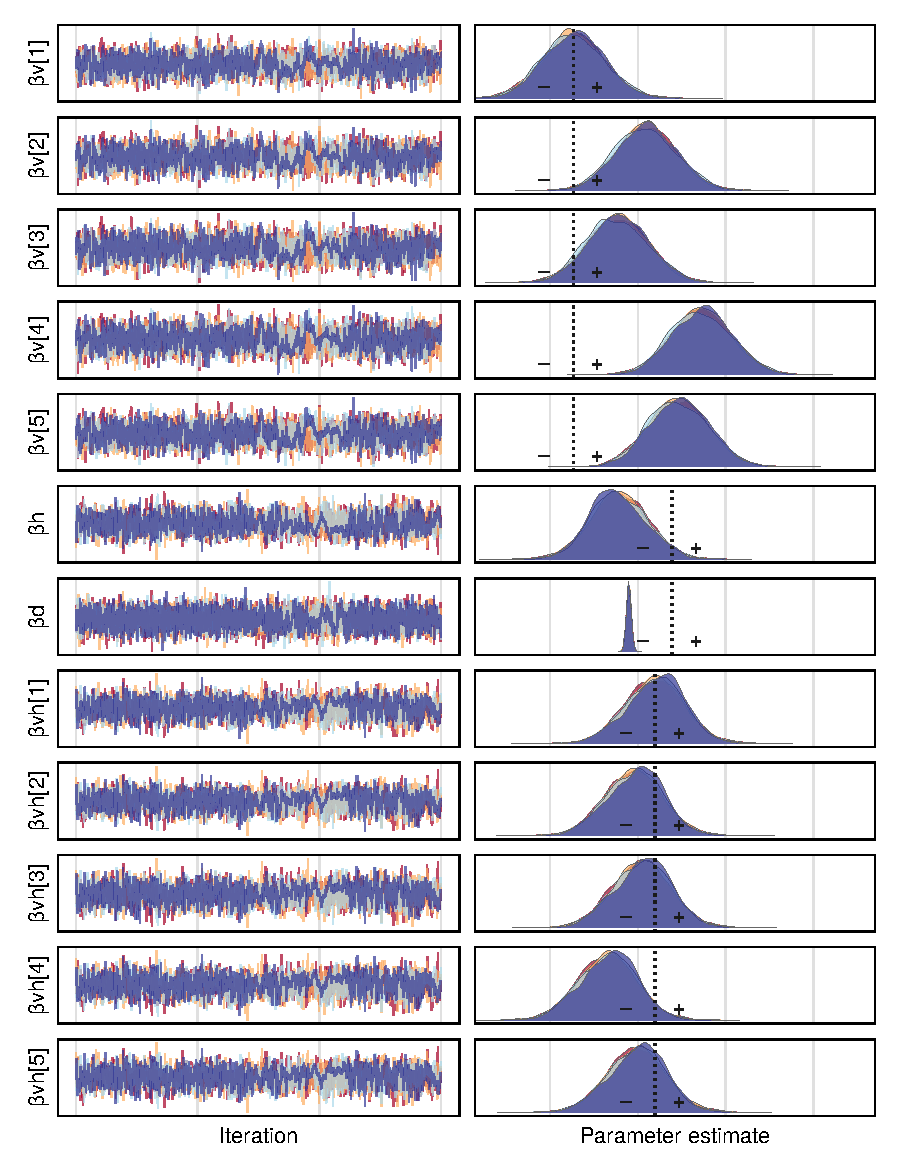
\includegraphics[width=0.7\textwidth, keepaspectratio=true]{./Figures/plots/IgG1_varint.pdf}
    \caption{MCMC chains and posterior distributions of coefficients for Diet, Habitat, Time post immunisation, and vaccine formulations A, AD, D, DA, and DD.}

    \label{supfig:igg1}

  \end{figure}
}

%%%%%%%%% TABLES

% \newcommand{\TblIndep}{
%     \begin{table}[htbp]
%         \centering
%         \begin{tabular}{ccccccc}
%             \hline
%                 & Coef. & Std. Error &   z &Pr(>|z|) & Lower 95\% & Upper 95\% \\
%             \hline
%     (Intercept) & -18.01 & 275.646 & -0.07 &  0.948 & -558.262  &  522.251 \\
%     V           &  1.199 &   1.031 &  1.16 &  0.245 &   -0.823  &    3.220 \\
%     D           & -1.917 &   0.923 & -2.08 &  0.038 &   -3.726  &   -0.108 \\
%     R           &  1.497 &   1.033 &  1.45 &  0.147 &   -0.528  &    3.521 \\
%     S           &  1.752 &   0.993 &  1.76 &  0.078 &   -0.194  &    3.698 \\
%     H           & 15.609 & 275.645 &  0.06 &  0.955 & -524.645  &  555.863 \\
%             \hline
%         \end{tabular}
%         \caption{GLM (\(P \upmodels V \mid D, R, S, H\))}
%         \label{table:implied_indep}
%     \end{table}

% }

\newcommand{\TblPrecis}{
  \begin{table}[htbp]
    \centering
    \caption{Posterior predictions of model parameters for random intercept Gaussian model \(E \sim Normal(\alpha[ID] + H + D + V + V:H, \sigma)\).}
    \sffamily
    \begin{tabular}{|>{\bfseries}l|ccccc|}
      \hline
      Parameter & \textbf{Mean} & \textbf{Std} & \textbf{5\%} & \textbf{50\%} & \textbf{95\%} \\
      \hline
      Intercept & 1.02          & 0.85         & -0.39        & 1.032         & 2.43          \\
      Habitat   & -0.519        & 0.806        & -1.863       & -0.513        & 0.795         \\
      Diet      & -0.253        & 0.072        & -0.373       & -0.253        & -0.137        \\
      A         & 0.0           & 0.871        & -3.307       & -1.892        & -0.438        \\
      D         & 2.062         & 0.856        & -1.228       & 0.175         & 1.598         \\
      AD        & 1.256         & 0.875        & -2.061       & -0.651        & 0.84          \\
      DA        & 3.652         & 0.87         & 0.343        & 1.751         & 3.215         \\
      DD        & 2.996         & 0.865        & -0.304       & 1.091         & 2.534         \\
      A:H       & 0.0           & 0.818        & -0.864       & 0.47          & 1.831         \\
      D:H       & -0.594        & 0.811        & -1.434       & -0.125        & 1.223         \\
      AD:H      & -0.371        & 0.823        & -1.244       & 0.103         & 1.472         \\
      DA:H      & -1.348        & 0.818        & -2.228       & -0.874        & 0.496         \\
      DD:H      & -0.527        & 0.818        & -1.389       & -0.061        & 1.31          \\

      \hline
    \end{tabular}
    \label{tbl:precis}
  \end{table}
}
